% \documentclass[twoside,twocolumn]{ujarticle}
\documentclass[titlepage]{jarticle}
%\usepackage{type1cm}
\usepackage{outline-ec}
\usepackage{amsmath,amssymb,verbatim,ascmac,multicol}
\usepackage{tabularx}
\usepackage[hang,small,bf]{caption}
\usepackage[subrefformat=parens]{subcaption}
\captionsetup{compatibility=false}
%\usepackage{multirow}
% dvioutで確認する場合は以下を有効にする
%\usepackage[dviout]{graphicx,color}
% pdf化する場合は以下を有効にする
\usepackage[dvipdfmx]{graphicx,color}
%
% --------------------------------------------------------------------------
% 図表番号の後の:を削除
%
\makeatletter
\long\def\@makecaption#1#2{% #1=図表番号,#2=キャプション本文
\sbox\@tempboxa{#1 \hskip0.5zw #2}% 図表番号とキャプションの間のスペース 0.5zw
\ifdim \wd\@tempboxa >\hsize
#1 #2\par 
\else
\hb@xt@\hsize{\hfil\box\@tempboxa\hfil}
\fi}
\makeatother
% --------------------------------------------------------------------------

%
% --------------------------------------------------------------------------
% 下の該当する部分を書き換える
%
\氏名{本間 三暉}			%% 自分の氏名
\出席番号{35}					%% 出席番号
\研究室名{視覚情報処理研究室}			%% 研究室名
\指導教官{高橋 章}			%% 指導教員名
%
% --------------------------------------------------------------------------
% 研究題目等
%
% 研究題目が2行になるときは \\ で行送りできる
%
\発表番号{B\;--\;2}
\研究題目{単一視点による人物の全身運動の三次元計測について}

% --------------------------------------------------------------------------
% アブストラクト
%
\アブストラクト{
全身運動を行う人物を一台のRGBカメラやRGBDカメラで撮影し,それぞれのカメラに合った画像処理を用いた手法で三次元骨格推定を行う.
そうして取得した三次元骨格推定の結果を精度や処理速度などについて比較し分析する.
% また,組み込みPCで実装する場合やカメラに対し手前にある物体が後ろにある物体を隠す状態になり十分に計測できないオクルージョンへの対応,
% リアルタイム処理を目的とした高速化を目指す.
% =======
% モーションキャプチャデバイスmocopiでは表現しきれない部分を画像処理を用いて補助することを検討する.
% mocopiでは関節部などが正確に計測できないことがあるため,竹馬や一輪車などの精密な重心移動や姿勢制御が必要な運動に関して測定を行い,
% 画像処理による骨格推定を組み合わせ,バランス運動時の重心や姿勢を解析することによって,mocopiの測定精度を上げることを目指す.
}
%
% --------------------------------------------------------------------------
% 本文開始
%
\begin{document}
\maketitle

%
% --------------------------------------------------------------------------
% 第1節
%
\section{研究背景・目的}
%
情報通信技術の急速な進歩により人工現実感,拡張現実感,複合現実感などの応用が広がっている.
感染症対策を契機にオンラインコミュニケーションも増加し,インターネット上の仮想共有空間であるメタバースが注目されている\cite{meta}.
その理由の一つに,離れている相手にテキストや音声だけでなく身振りや動作などのノンバーバルな情報の伝達を行うことが容易であるという点がある.

三次元の仮想空間で自分の分身となるアバターを自由に操作するには,
体の動きを計測する必要があり,画像処理による方法\cite{CV}や専用デバイスを装着する方法\cite{キャプチャ}などが試みられている.
画像処理による方法で三次元の情報を取得するためには先行研究のような複数台のカメラを用いる方法\cite{turugi}があるが,狭い室内であるなどの場所の制約や,
限られた予算の中で実装したいという資金の制約などによって,複数台のカメラを用いる方法取るのが難しい場合がある.
また,機械学習を用いることで一台のカメラや少ないセンサでも三次元骨格推定を可能にするオープンソースが増えている.

本研究では1台の入力装置で三次元骨格推定ができる現行の方法について調査及び実装を行い, % ここ書き換えたいかも
動作の緩急やオクルージョンという自分の体に体の一部が隠れてしまい計測の信頼度が下がってしまう状態の有無について,
それぞれの方法の精度を定量的に比較する.
% --------------------------------------------------------------------------
% 第2節
%
\section{研究内容}
%これって研究背景に描いたほうが自然か?

%
% --------------------------------------------------------------------------
% 第2節 第1小節
%
\subsection{人の動作の計測方法}
%
人の動作の三次元計測を行うには,画像処理による方法やモーションセンサによる方法がある.それぞれの方法について簡単にまとめたものを表\ref{3D_1}に示す.
画像処理による方法では画像から人の骨格を推定することで人の動作を解析できる.
画像処理による三次元骨格推定は撮影するカメラに,色情報を記録できる一般的なRGBカメラを用いて解析する方法と,
カメラと物体の距離を測ることができるRGBDカメラ用いて解析する方法がある.
% これらの方法はモーションセンサを用いるものと比べると精度にばらつきが生まれる.

%% モーションセンサのしゅるいについてもかいたほうが自然か?
% モーションセンサによる方法は光学式や慣性式などがあるが,どの方法も精度が高いかわりにマーカーやセンサを検出対象に取り付けなければならないため使用できる環境が限定されてしまう.
モーションセンサによる方法は,光学式や慣性式などがある.
光学式は体表面にマーカーを取り付けそのマーカーを複数台のカメラで取り込むことで骨格を推定する.
慣性式は加速度,角速度,方位を測定できるセンサを体表面の指定箇所に取り付けることで骨格を推定する.


\begin{table}[t!]
  \centering
  \caption{動作を計測する方法の種類と特徴}
  \begin{tabular}{l|ll|ll}
    \hline
                  & \multicolumn{2}{c|}{\small{カメラ}}       & \multicolumn{2}{c}{\small{モーションセンサ}}                                                     \\ \cline{2-5}
                  & \multicolumn{1}{c|}{\small{RGB}}       & \small{RGBD}                         & \multicolumn{1}{c|}{\small{光学式}} & \small{慣性式}    \\ \hline
    \small{センサ装着} & \multicolumn{1}{c|}{\small{不要}}        & \small{不要}                           & \multicolumn{1}{c|}{\small{必要}}  & \small{必要}     \\
    \small{外から撮影} & \multicolumn{1}{c|}{\small{必要}}        & \small{必要}                           & \multicolumn{1}{c|}{\small{必要}}  & \small{不要}     \\
    \small{必要台数}  & \multicolumn{1}{c|}{\small{1$\sim$数台}} & \small{1台}                           & \multicolumn{1}{c|}{\small{複数台}} & \small{0台}     \\ \hline
    \small{計測方法}  & \multicolumn{1}{c|}{\small{MediaPipe}} & \small{Nuitrack}                     & \multicolumn{1}{c|}{\small{}}    & \small{mocopi} \\%%%これも怪しいけどね
    \small{計測関節数} & \multicolumn{1}{c|}{\small{33個}}       & \small{19個}                          & \multicolumn{1}{c|}{\small{}}    & \small{27個}    \\
    \hline
  \end{tabular}
  \label{3D_1}
\end{table}
%
% --------------------------------------------------------------------------
% 第2節 第2小節
%
\subsection{RGBカメラ一台を用いた三次元骨格推定}
%
一台のRGBカメラで撮影した動画から骨格推定を行う場合,
MediaPipe Pose\cite{mediapipe}というライブラリを用いて処理することで骨格推定が行える.

MediaPipeはGoogleが提供しているライブメディアやストリーミングメディア向けの機械学習ソリューションである.
特徴として,顔認識や物体検出などが行えるライブラリがあり,計算コストが低くスマートフォンや組み込みPCなど資源の限られたハードウェアでも使用できるという点が挙げられる.%%%この辺怪しい
また,その中でもMediaPipe Poseは動画から人間の姿勢を推論するライブラリで,
動画から
% 図\ref{RGB}に示す
全身の33個の関節の三次元位置または上半身の25個の関節の三次元位置を予測できる.

\begin{figure*}[t]
  \begin{tabular}{cc}
    \begin{minipage}[]{0.3\hsize}
      \centering
      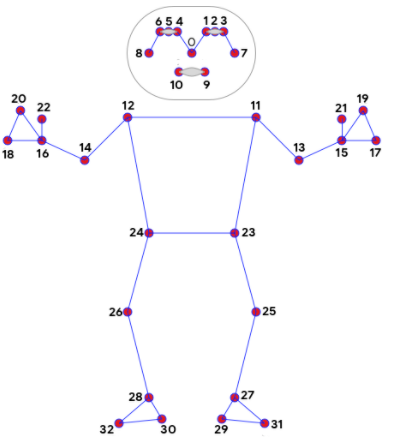
\includegraphics[height=45mm]{img/media.png}
      \subcaption{MediaPipe Poseで取得できる関節位置}
      \label{RGB} %%%後で変える
    \end{minipage}
    \hspace{0.03\columnwidth} % ここで隙間作成
    \begin{minipage}[]{0.3\hsize}
      \centering
      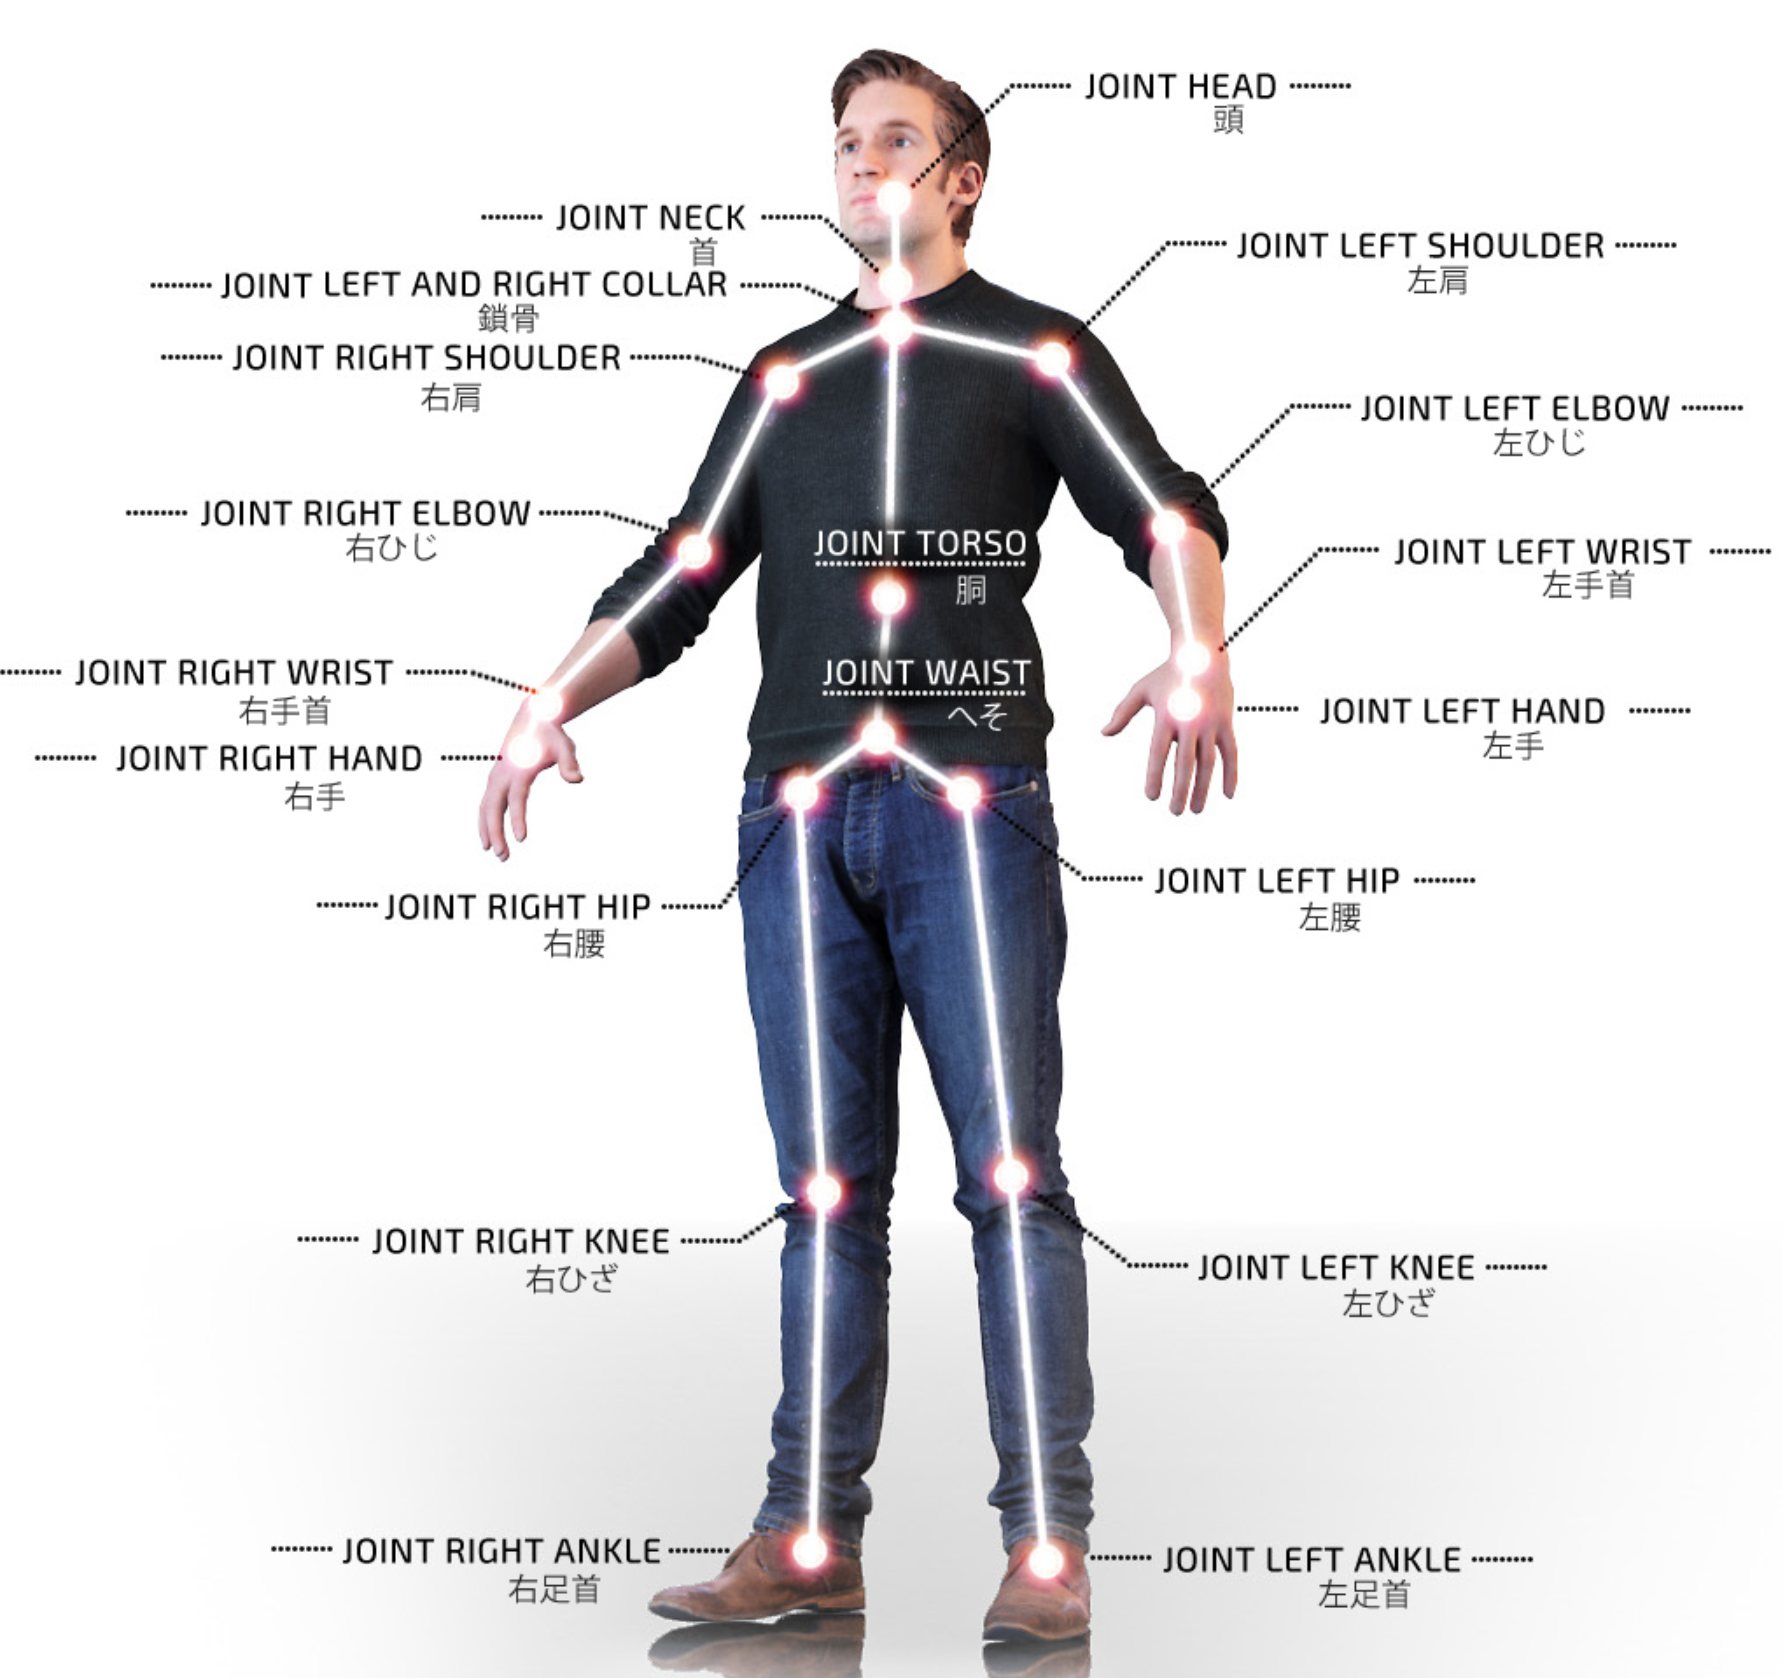
\includegraphics[height=45mm]{img/nuitrack.png}
      \subcaption{Nuitrackで取得できる関節位置}
      \label{RGBD} %%%後で変える
    \end{minipage}
    \hspace{0.03\columnwidth} % ここで隙間作成
    \begin{minipage}[]{0.3\hsize}
      \centering
      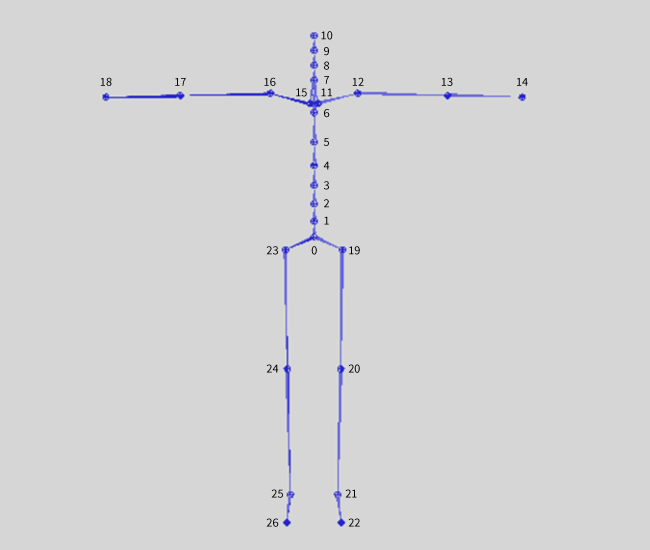
\includegraphics[height=45mm]{img/TechSpec_02.png}
      \subcaption{mocopiで取得できる関節位置}
      \label{mocopi} %%%後で変える
    \end{minipage}
    \caption{取得できる骨格}
  \end{tabular}
\end{figure*}

\subsection{RGBDカメラで行う三次元骨格推定}
% 入力をRGBDカメラにする場合,kinectSDK\cite{kinectSDK}などのハードウェアの公式から出ているソフトウェアやOpenNI\cite{openni}などのオープンソースを処理に用いることによって三次元骨格推定を行うことができる.
% RGBDカメラを入力装置として用いる際の関係を図\ref{app}に示す.
kinectSDK\cite{kinectSDK}のようなデバイス専用のソフトウェアや,Nuitrack\cite{nuitrack}などのオープンソースを開発ライブラリに用いて処理することによってアプリケーションを作成できる.

% \begin{figure*}[t!]
% \centering
% 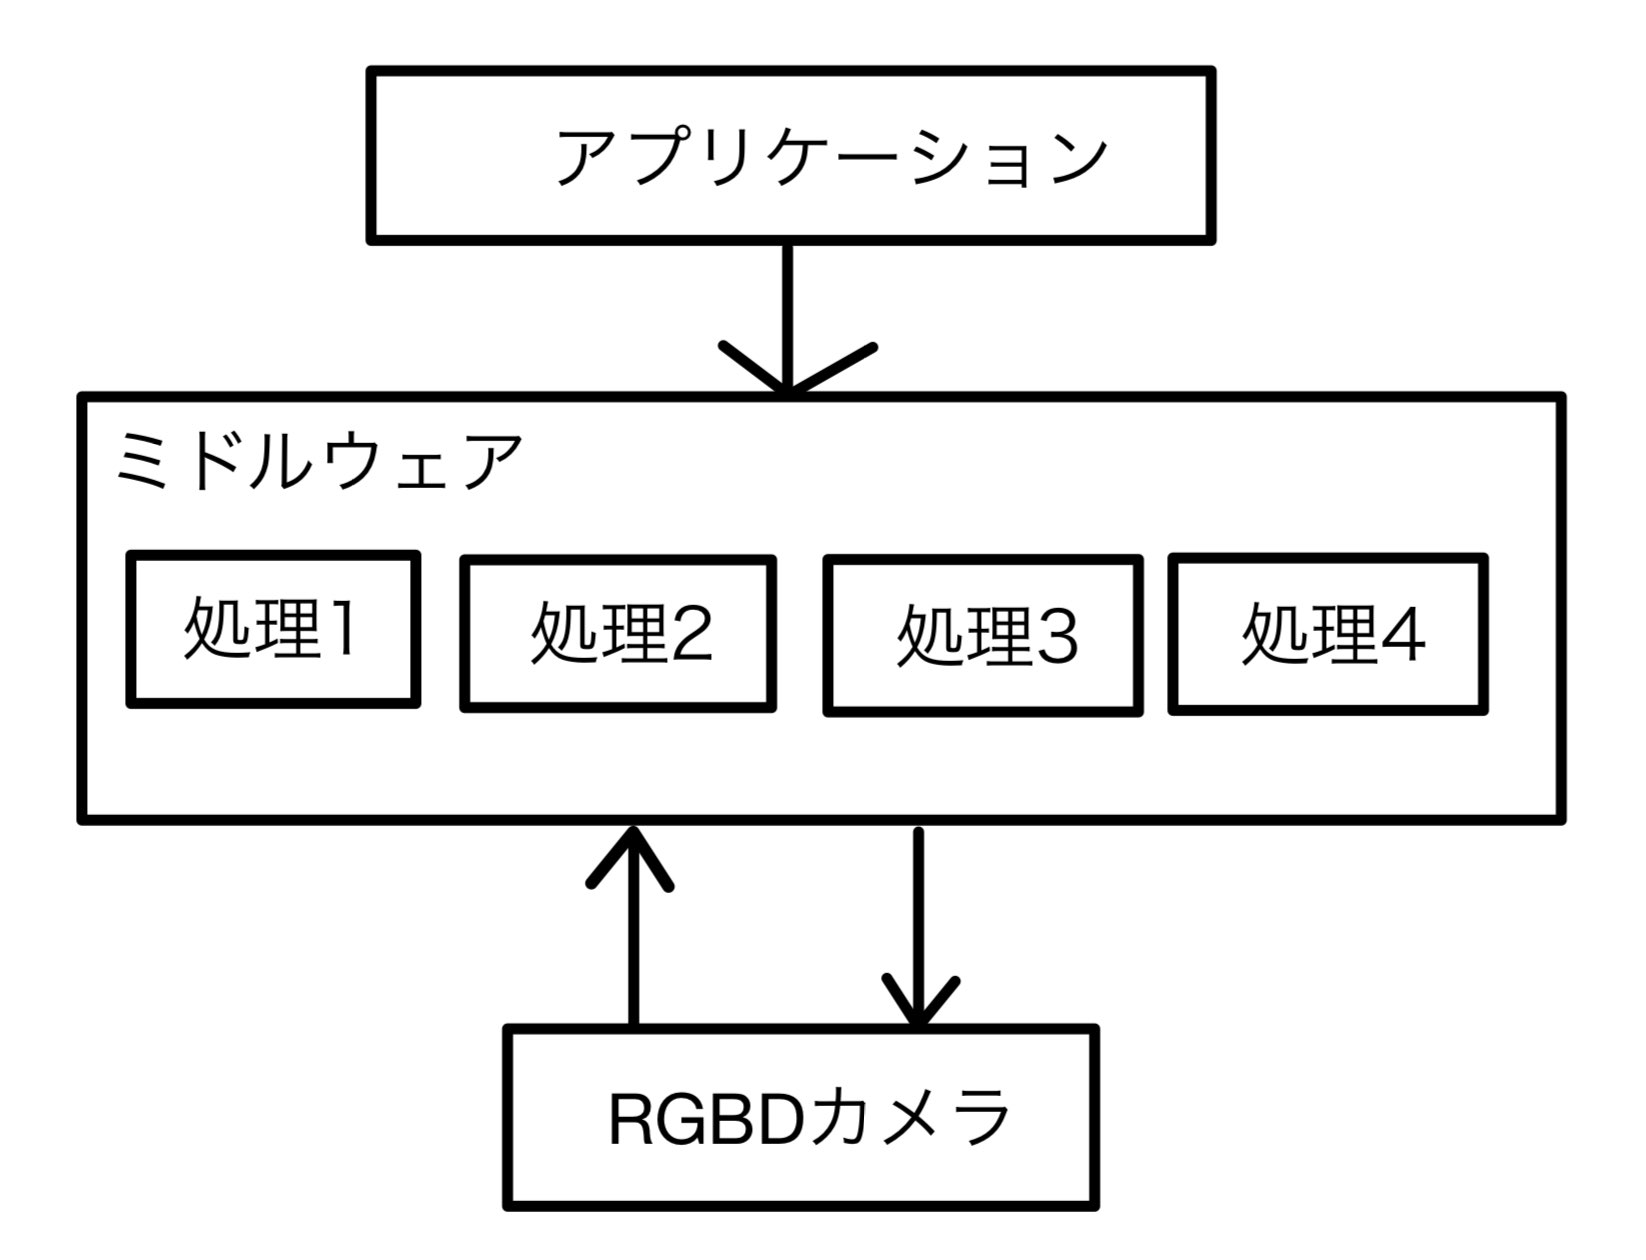
\includegraphics[width=6cm]{img/app3.jpg}
% \caption{RGBDカメラを入力装置として用いる際の関係}
% \label{app}
% \end{figure}

代表的なRGBDカメラと開発ライブラリの組み合わせを表\ref{RGBD}に示す.

% \begin{table}[t!]
%   \centering
%   \caption{RGBDカメラと開発ライブラリの組み合わせ}
%   \begin{tabular}{l|l}\hline
%     カメラ       & 開発ライブラリ          \\\hline
%     kinect2   & kinectSDK,OpenNI \\
%     RealSense & Nuitrack         \\\hline
%   \end{tabular}
%   \label{RGBD}
% \end{table}

% kinectSDKはMicrosoft Kinect for Windows Software Development Kit の略で,Microsoft社から公式にリリースされた開発キットである.
% Windows上でkinect2を動かすのに必要なドライバやドキュメントなどが同梱されている.
% kinectSDKはハードウェアであるkinect2との組み合わせに限定されており,現在は開発が終了してしまっている.

% kinectSDKと似たような機能を持つもので,Kinectのセンサ部分を開発したPrimeSense社が中心となって開発したOpenNIというライブラリがある.
% % OpenNIの構成を図\ref{app}に示す.
% OpenNIには部分的なトラッキングやジェスチャ検出機能などkinectSDKに比べできることが多く,GitHub上でソースコードが公開されており現在も有志による開発が行われている.

% % kinect2で撮影する場合はkinectSDKやOpenNIを用いて解析することで三次元骨格推定を行うことができるが,kinectSDKとOpenNIの両方に長所と短所があるためそれぞれの場合について実装し比較を行う.

本研究で扱うNuitrackは3DiVi Incが開発した三次元トラッキングミドルウェアで,RealSense D400シリーズやOrbbec Astraシリーズ等のRGBDカメラで骨格推定が可能であり,
全身の19個の関節部分のトラッキングが可能である.
%
% --------------------------------------------------------------------------
% 第2節 第3小節
%
\subsection{慣性式モーションキャプチャによる三次元骨格推定}
%
画像処理の精度を比較する際,画像処理による方法で取得したデータを基準にするのは特定の骨格推定の方法に有利な結果が出てしまう可能性がある.
そのため,基準とするデータは画像処理に頼らない独立した方法で取得する必要があるなどの理由からモーションキャプチャデバイスmocopi\cite{mocopi}を用いる.

mocopiとは,市販のモーションキャプチャデバイスで両手,両足,頭,腰の計6か所に小型センサを装着してリアルタイムに三次元計測を行うことができる.
6つの小型センサで測定しているため肘や膝などの関節部の屈曲を正確に表現することはできないが,mocopiのセンサはそれぞれ3つの自由度を持つ加速度センサと角度センサで測定しており,
機械学習を用いることで,肘や膝などの関節部を含めた全身の推定を実現している.
%
% --------------------------------------------------------------------------
% 第2節 第4小節
%
\subsection{キャリブレーション}
%
計測方法によりスケール,処理により発生する遅延によるフレームのズレ,座標系が違うため統一しなければ定量的な比較が行えない.
そのため,これらを統一するためのキャリブレーションを行う必要がある.

キャリブレーションの方法として,計測する運動をする前に両手を水平に広げその時の両手首の長さを元にスケールを合わせる.
次に,両手を合わせ両手首の座標が最接近した時点を基準としてフレームのズレを合わせる.
最後に,へその座標を原点として頭に向かう方向をz軸,右手首から左手首に向かう方向をx軸,これらの軸と直行する方向をy軸として座標系を定める.
%
% --------------------------------------------------------------------------
% 第2節 第5小節
%
% \subsection{結果}
% %
% 右手首の結果を表\ref{righthand}に示す.

% \begin{table}[b!]
%   \centering
%   \caption{右手首の基準と測定値の差分}
%   \begin{tabular}{c|c||c|c}
%                             &           & RGB & RGBD \\\hline\hline
%     \multirow{2}{*}{動作が緩やか} & オクルージョンなし &     &      \\
%                             & オクルージョンあり &     &      \\\hline
%     \multirow{2}{*}{動作が急}   & オクルージョンなし &     &      \\
%                             & オクルージョンあり &     &      \\\hline
%   \end{tabular}
%   \label{righthand}
% \end{table}
\begin{table}[b!]
  \centering
  \caption{右手首の基準と測定値の差分}
  \begin{tabular}{c||c|c|c|c}
            & \multicolumn{2}{l}{動作が緩やか} & \multicolumn{2}{l}{動作が急}           \\\hline
    オクルージョン & なし                         & あり                       & なし & あり \\\hline\hline
    RGB     &                            &                          &    &    \\
    RGBD    &                            &                          &    &    \\\hline
  \end{tabular}
  \label{righthand}
\end{table}
%
%
%
% --------------------------------------------------------------------------
% 第2節 第6小節
%
%\subsection{}
%

%
%
%
% --------------------------------------------------------------------------
% 第3節
%
\section{研究結果}
%


%
% --------------------------------------------------------------------------
% 第3節 第1小節
%
\subsection{実験方法}
%
% mocopiを装着して学校体操をしている人をRGBカメラ,kinect2,RealSenseで同時に撮影する.
% それぞれのカメラで撮影した映像から三次元骨格推定を行い,推定した骨格とmocopiで測定した骨格の両手,両足,頭,腰の座標のズレを誤差として精度の計測を行う.
mocopiを装着し,
%
%
% --------------------------------------------------------------------------
% 第3節 第2小節
%
\subsection{実験結果}
%
% ・撮影機材や開発環境について記述
% 本研究では,開発環境としてmocopiとOpenPoseを使用する.

%
%


%
%
% --------------------------------------------------------------------------
% 第3節 第3小節
%
% \subsection{進捗状況}
%
%
% --------------------------------------------------------------------------
% 第3節 第4小節
%
%\subsection{}
%

%

%
%
% --------------------------------------------------------------------------
% 第4節
%
\section{まとめ}
%

% 学校体操や空手の型などの,体を大きく動かし,関節の位置や体の相対関係が正しく測定できるようにする.
%
% --------------------------------------------------------------------------
% 参考文献
%

\begin{thebibliography}{99}
  \small{
    \bibitem{meta}{
      日本経済新聞,``孤独感抱える若者の交流の場,メタバースに開設'',https://onl.la/Y7BehPP
    }
    \bibitem{CV}{
      平尾 公男ら,``多関節 CG モデルと距離画像による上半身の姿勢推定'',Technical report of IEICE.
      PRMU, VOL.104, No.573, 79--84, 2004.
    }
    \bibitem{キャプチャ}{
      白鳥 貴亮ら,``モーションキャプチャと音楽情報を用いた舞踊動作解析手法'',電子情報通信学会論文誌D,Vol.J88-D2,No.8,pp.1662-1671,2005.
    }
    \bibitem{turugi}{
      剱 一輝,``柔道競技の3Dアーカイブ化'',令和4年度長岡高専専攻科論文,2023.
    }
    % \bibitem{baseline}{
    %   J. Martinez, R. Hossain, J. Romero, J. Little. ``A simple
    %   yet effective baseline for 3d human pose estimation'' . In
    %   ICCV, 2017.
    % }
    \bibitem{ビデオ}{
      安達 康平ら,``ビデオからの3次元姿勢を用いた行動認識における精度向上の試み'',研究報告モバイルコンピューティングとパーベイシブシステム(MBL),
      2020-MBL-94,47,1--7,2020.
    }
    \bibitem{kinectSDK}{
      谷尻 豊寿,``体の動きがコントローラ C++でkinectプログラミング KINECTセンサ画像処理プログラミング'',株式会社 カットシステム,2011.
    }
    \bibitem{nuitrack}{
      3DiVi Inc,``Nuitrack'',https://nuitrack.com/jp
    }
    \bibitem{mediapipe}{
      Google,``mediapipe'',https://developers.google.com/mediapipe
    }
    \bibitem{mocopi}{
      SONY,``モバイルモーションキャプチャーmocopi'',https://www.sony.jp/mocopi/
    }
    % \bibitem{openpose}{
    %   CAO,Zhe,et al.OpenPose: Realtime Multi-Person 2D Pose Estimation Using Part Affinity Fields. arXiv preprint arXiv:1812.08008. 2018.
    % }
  }
\end{thebibliography}
\rightline{URLは2023年10月4日にアクセス}
\end{document}
